\section{Overall \ac{REACT}  Framework}
\label{sec:framework}
\ac{REACT} framework, as depicted in \ref{fig:abstract}, consists of two main components: an offline planning phase and an online execution phase. In the offline phase, the environment is provided as a point cloud, including the object to be inspected. Then, a \ac{SDF} map is generated from this point cloud using the nvblox library \cite{nvblox}. Subsequently, the extracted point cloud of the structure under inspection is processed via FC-Planner \cite{feng2024fc} to compute an optimal waypoint sequence, generating a path that renders full inspection coverage while disregarding the tether constraints.

%Online Phase
In the online phase, tether constraints are handled by an entanglement-aware replanner that ensures that the maximum tether length is not exceeded due to entanglement. This is achieved using our developed tether model, which continuously updates based on the current state of the tether and the new position of the \ac{ROV}, denoted as $\textbf{p}_{\mathrm{rov}}$. The online planner then provides the reference state to an \ac{MPC} controller, which computes and applies the optimal wrench (forces and torques) to the \ac{ROV}.



%%%%%%%%%%%%%%%%%%%%%
%%%%%%  Tether Figure  
%%%%%%%%%%%%%%%%%%%%%

\begin{figure*}[t!]
    \centering
    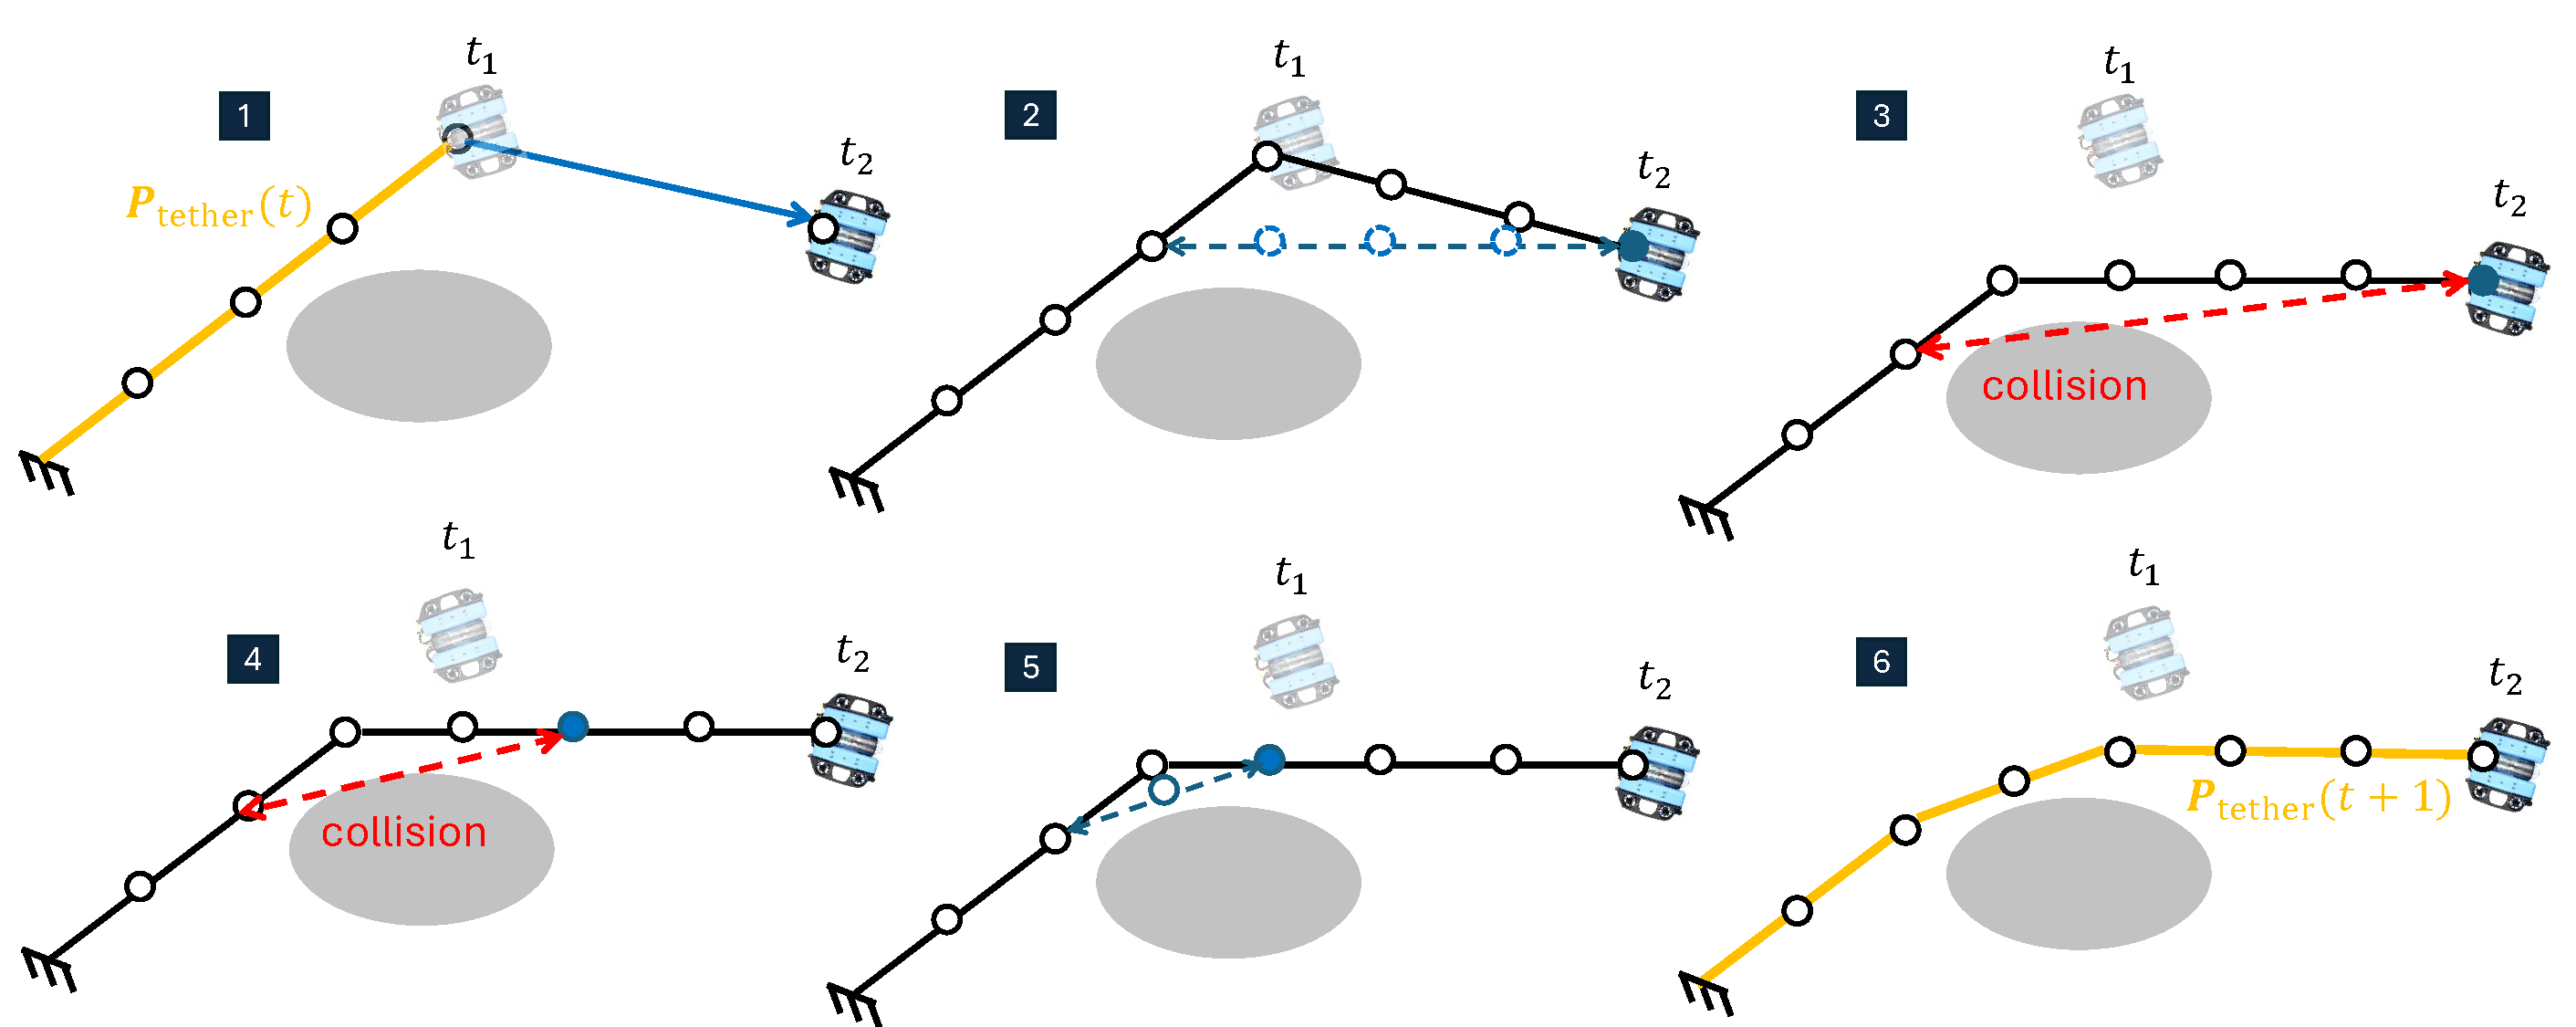
\includegraphics[width=1\linewidth]{EA-Planner/figures/tether_model.pdf}
    \caption{Tether shortcutting during \ac{ROV} motion from \( t_1 \) to \( t_2 \). (1) Initial tether with new \ac{ROV} position \( \mathbf{p}_{\text{rov}} \) appended; (2) Successful shortcut from the end node; (3) Collision encountered when attempting further shortcutting, prompting move to the next node; (4) Another collision detected from the new node; (5) Successful shortcut from a subsequent node; (6) Final tether configuration (yellow) after applying all feasible shortcuts.}
    \label{fig:tether}
\end{figure*}
%%%%%%%%%%%%%%%%%%%%%%%%



%%%%%%%%%%%%%%%%%%%%%%%%%%%
%%%%%%%%%%%%%%%%%%%%%%%%%%%
%%%%%% Tether Model Section
%%%%%%%%%%%%%%%%%%%%%%%%%%%
%%%%%%%%%%%%%%%%%%%%%%%%%%%
\section{Tether Modeling}
\label{sec:tether_model}
%Next, we introduce a computationally efficient kinematic \ac{ROV} tether model, inspired by the shortcutting algorithm used in the ropeRRT path planner \cite{roperrt}. In essence, the proposed model predicts the position of each node along the tether length based on \ac{ROV}'s relative pose to the base. 
%which simplifies sampled trajectories in a manner analogous to a rope tightening around an obstacle. The key assumption in the proposed model is that we assume a geometry-based constraint where the tether remains taut and fully stretched at all times.

 We introduce a computationally efficient kinematic tether model for tethered underwater vehicles. This model predicts the tether path, specifically the positions of each node along the tether's length, based on the \ac{ROV}'s relative pose to the base, and assumes a geometry-based constraint where the tether remains taut and fully stretched at all times. The main idea of the proposed tether model is inspired by the shortcutting algorithm of the ropeRRT path planner \cite{roperrt}, which simplifies sampled trajectories similar to a rope tightening around an obstacle. 


\subsection{Tether model description}
Let the tether path at time \( t \) be denoted by \( \mathbf{P}_{\mathrm{tether}}(t) = \{ \mathbf{p}_i(t) \}_{i=1}^{N} \), where each node \( \mathbf{p}_i(t) \in \mathbb{R}^3 \) represents the position of the \( i \)-th node in 3D space at time \( t \), and \( N \) is the total number of nodes in the tether path. The \ac{ROV} position at time \( t \), denoted by \( \mathbf{p}_{\mathrm{rov}}(t) \in \mathbb{R}^3 \), is appended at the end \( \mathbf{p}_{N+1}(t) \), ensuring that the \ac{ROV}'s position is included in the tether path. 

The proposed tether model iteratively optimizes the tether path via two primary mechanisms: shortcutting and pulling. %, as illustrated in Fig.~\ref{fig:tether}. 
%For each pair of nodes \( (\mathbf{p}_i(t), \mathbf{p}_j(t)) \) where \( i < j \), the algorithm attempts to shortcut the path segment between them.
Starting at the last node ($\mathbf{p}_j(t) = \mathbf{p}_{N}(t)$), the algorithm attempts to shortcut the path segment between each pair of nodes \( (\mathbf{p}_i(t), \mathbf{p}_j(t)) \) where \( i < j \).
If the line of sight between \( \mathbf{p}_i(t) \) and \( \mathbf{p}_j(t) \) is collision-free, as determined via an \ac{SDF} map (\( \mathcal{M}_{sdf} \)), the intermediate nodes are replaced with a straight segment sampled at known resolution \( \delta_n \). Conversely, if the line of sight encounters a collision, $j$ shifts to the preceding node, and the collision-free line of sight is rechecked. This process is repeated until a collision-free line of sight is found, and the intermediate nodes are then replaced. Fig.~\ref{fig:tether} illustrates an example of the shortcut operation. 

In the presence of non-convex obstacles, nodes might be positioned on or close to the obstacle following the shortcutting operation. Hence, if the shortcut is obstructed or the endpoint node \( \mathbf{p}_j(t) \) is in collision, the model applies a pulling operation. This operation essentially simulates disentanglement by moving \( \mathbf{p}_j(t) \) incrementally toward the tether endpoint \( \mathbf{p}_{N+1}(t) \), thus ensuring a collision-free updated path. This iterative process continues until no further shortcuts or pulling is feasible, resulting in an updated, taut, and obstacle-free tether path \( \mathbf{P}_{\mathrm{tether}}(t+1) \). Both the shortcutting and pulling operations are described in algorithm~\ref{alg:tether_optimization}.



%%%%%%%%%%%%%%%%%%%%%%%%%%%%%%%%%%%%%%%%%%
%%%%%%  Tether Model Algorithm  %%%%%%%%%
%%%%%%%%%%%%%%%%%%%%%%%%%%%%%%%%%%%%%%%%%%


\begin{algorithm}[t]
%\SetAlgoLined
\LinesNotNumbered  % Disable line numbers

\SetKwInOut{Input}{Require}
\SetKwInOut{Output}{Return}
\Input{
ROV position $\mathbf{p}_{\mathrm{rov}}(t)$, 
Tether path $\mathbf{P}_{\mathrm{tether}}(t)$, 
SDF map $\mathcal{M}_{sdf}$, 
parameters: $\delta_{n}$
}
\Output{Taut-tether at $t+1$ : $\mathbf{P}_{\mathrm{tether}}(t+1)$}
\BlankLine

\tcp{Extend tether path to include the current ROV position as the endpoint}
Append $\mathbf{p}_{\mathrm{rov}}(t)$ to $\mathbf{P}_{\mathrm{tether}}(t).end()$\;

%\tcp{Iterative shortcutting path segments by skipping intermediate nodes}
\tcp{Iterative shortcutting}
\For{$i \gets len(\mathbf{P}_{\mathrm{tether}}(t)) - 2$ \textbf{to} $1$}{
    \For{$j \gets i+1$ \textbf{to} $len(\mathbf{P}_{\mathrm{tether}}(t)) - 1$}{
        \tcp{Check if shortcutting the path is valid between nodes $i$ and $j$}
        \If{checkShortcut($\mathbf{P}_{\mathrm{tether}}(t), i, j$)}{
            \tcp{Replace intermediate nodes $i-j$ }
            replaceNodes($\mathbf{P}_{\mathrm{tether}}(t)$, $i$, $j$, $\delta_{n}$)\;
        }
        \Else{
            \If{not checkLineOfSight($\mathcal{M}_{sdf}$, $\mathbf{P}_{\mathrm{tether}}(t)$)}{
                \tcp{Line of sight is blocked by obstacle, stop shortcutting}
                \textbf{break}\;
            }
            \If{isInCollision($\mathcal{M}_{sdf}$, $\mathbf{P}_{\mathrm{tether}}(t)[j]$)}{
                \tcp{Pull node towards tether end}
                pullNode($\mathbf{P}_{\mathrm{tether}}(t)[j]$, $\mathbf{P}_{\mathrm{tether}}(t).end()$, $\delta_{n}$)\;
            }
        }
    }
}
\Return{$\mathbf{P}_{\mathrm{tether}}(t+1)$}\;
\caption{Taut-Tether Model}
\label{alg:tether_optimization}
\end{algorithm}




%%%%%%%%%%%%%%%%%%%%%%%%%%%
%%%%%%%%%%%%%%%%%%%%%%%%%%%
% Homotopy equivelance proof
%%%%%%%%%%%%%%%%%%%%%%%%%%%
%%%%%%%%%%%%%%%%%%%%%%%%%%%


% \subsection{Homotopic Equivalence of the Shortcutting-Based Tether Path}
% \label{sec:homotopy_proof}

% In this subsection, we demonstrate that the taut-tether path generated primarily through the shortcutting mechanism is homotopically equivalent to the Remotely Operated Vehicle's (ROV) actual trajectory. This argument focuses on the geometric simplification provided by shortcutting, assuming the tether behaves like a rope tightening around obstacles.

% \subsubsection{Preliminaries and Definitions}
% Let the ambient Euclidean space be $X = \mathbb{R}^3$. The static obstacle region, $O \subset X$, is a closed set. The \textbf{free configuration space} is defined as $C_{free} = X \setminus O$. A \textbf{path} in $C_{free}$ is a continuous function $\gamma: [0,1] \to C_{free}$.

% Two paths $\gamma_0, \gamma_1: [0,1] \to C_{free}$ sharing the same endpoints (i.e., $\gamma_0(0)=\gamma_1(0)$ and $\gamma_0(1)=\gamma_1(1)$) are said to be \textbf{homotopic in $C_{free}$} (denoted $\gamma_0 \sim \gamma_1$) if there exists a continuous function $H: [0,1] \times [0,1] \to C_{free}$, called a \textbf{homotopy}, such that:
% \begin{itemize}
%     \item $H(s,0) = \gamma_0(s)$ for all $s \in [0,1]$,
%     \item $H(s,1) = \gamma_1(s)$ for all $s \in [0,1]$,
%     \item $H(0,\tau) = \gamma_0(0)$ for all $\tau \in [0,1]$ (startpoints fixed),
%     \item $H(1,\tau) = \gamma_0(1)$ for all $\tau \in [0,1]$ (endpoints fixed).
% \end{itemize}
% Let $p_A \in C_{free}$ denote the fixed anchor point of the tether and $p_R(t) \in C_{free}$ be the ROV's position at time $t$. The actual continuous trajectory of the ROV up to time $t$ is a path $\Gamma_{\mathrm{rov}}: [0,1] \to C_{free}$, with $\Gamma_{\mathrm{rov}}(0) = p_A$ (assuming the path starts at the anchor for simplicity) and $\Gamma_{\mathrm{rov}}(1) = p_R(t)$.

% A \textbf{piecewise linear (PL) path}, $\mathbf{P}$, connecting $p_A$ to $p_R(t)$ is defined by an ordered sequence of $N+1$ vertices $(v_0, v_1, \ldots, v_N)$ where $v_0=p_A$, $v_N=p_R(t)$, and each $v_k \in C_{free}$. The path consists of line segments $L(v_k, v_{k+1}) = \{ (1-s)v_k + s v_{k+1} \mid s \in [0,1] \}$. For $\mathbf{P}$ to be a path in $C_{free}$, each segment $L(v_k, v_{k+1})$ must be entirely contained in $C_{free}$.

% \subsubsection{Initial Tether Path and Shortcutting as a Homotopy}
% Let $\mathbf{P}_{init}(t)$ be an initial PL path representing the tether before shortcutting optimization at time $t$. This path connects $p_A$ to $p_R(t)$ and is assumed to be a PL approximation of $\Gamma_{\mathrm{rov}}$ lying in $C_{free}$. It is a standard result in algebraic topology that $\Gamma_{\mathrm{rov}} \sim \mathbf{P}_{init}(t)$ if $\mathbf{P}_{init}(t)$ is a sufficiently fine approximation.

% The shortcutting mechanism iteratively refines a PL path. Let $\mathbf{P}_{k} = (v_0, \ldots, v_M)$ be the PL tether path at iteration $k$. A shortcutting step selects two non-consecutive vertices $v_i, v_j \in \mathbf{P}_{k}$ (where $i < j-1$). Let $\sigma_{old}$ be the subpath of $\mathbf{P}_{k}$ from $v_i$ to $v_j$, and let $\sigma_{new}$ be the straight-line segment $L(v_i, v_j)$. If $\sigma_{new} \subset C_{free}$ (i.e., the line of sight is collision-free), the path $\mathbf{P}_{k+1}$ is formed by replacing $\sigma_{old}$ with $\sigma_{new}$.

% \textbf{Claim:} If $\sigma_{new} \subset C_{free}$, then $\sigma_{old} \sim \sigma_{new}$ in $C_{free}$ relative to their common endpoints $v_i$ and $v_j$.

% \textit{Proof of Claim:}
% The tether model is "analogous to a rope tightening around an obstacle." When a flexible rope segment, initially following $\sigma_{old} \subset C_{free}$, is pulled taut between $v_i$ and $v_j$, and the direct path $\sigma_{new}$ is also in $C_{free}$, the rope physically deforms into $\sigma_{new}$ by moving exclusively through $C_{free}$.
% This continuous deformation can be represented by a homotopy. Let $\sigma_{old}(s)$ parameterize the PL path $\sigma_{old}$ for $s \in [0,1]$, and $\sigma_{new}(s) = (1-s)v_i + s v_j$ parameterize the segment $\sigma_{new}$. A straight-line homotopy is $H(s, \tau) = (1-\tau)\sigma_{old}(s) + \tau\sigma_{new}(s)$ for $s, \tau \in [0,1]$.
% The "rope tightening" analogy implies that if $\sigma_{new} \subset C_{free}$, then the entire region swept by the deformation from $\sigma_{old}$ to $\sigma_{new}$ is also contained in $C_{free}$. Thus, $H(s, \tau) \in C_{free}$ for all $s, \tau$. This ensures that $\sigma_{old} \sim \sigma_{new}$ in $C_{free}$.
% Since $\mathbf{P}_{k+1}$ is obtained from $\mathbf{P}_{k}$ by substituting $\sigma_{old}$ with a homotopic segment $\sigma_{new}$, it follows that $\mathbf{P}_{k} \sim \mathbf{P}_{k+1}$.
% \hfill $\qed$

% \subsubsection{Iterative Application and Final Equivalence}
% The shortcutting algorithm generates a sequence of PL paths $\mathbf{P}_{init}(t) = \mathbf{P}_0, \mathbf{P}_1, \ldots, \mathbf{P}_{final}$, where $\mathbf{P}_{final}$ is the resulting taut-tether path, denoted $\mathbf{P}^{tether}(t)$. Since each step is a homotopy, $\mathbf{P}_0 \sim \mathbf{P}_1 \sim \ldots \sim \mathbf{P}_{final}$. By the transitivity of the homotopy relation, $\mathbf{P}_{init}(t) \sim \mathbf{P}^{tether}(t)$.

% Given that $\Gamma_{\mathrm{rov}} \sim \mathbf{P}_{init}(t)$, and $\mathbf{P}_{init}(t) \sim \mathbf{P}^{tether}(t)$, we conclude by transitivity that:
% $$ \Gamma_{\mathrm{rov}} \sim \mathbf{P}^{tether}(t) $$
% Thus, the taut-tether path $\mathbf{P}^{tether}(t)$, resulting from the shortcutting operations, is homotopically equivalent to the ROV's actual trajectory $\Gamma_{\mathrm{rov}}$ within the free configuration space $C_{free}$. The shortcutting process simplifies the path to a tighter representative within its original homotopy class with respect to the obstacles.



%%%%%%%%%%%%%%%%%%%%%%%%%%%%%%%%%%%%%%%%%%
%%%%%%%%%%%%%%%%%%%%%%%%%%%%%%%%%%%%%%%%%%
%%%%%%%%%%%%%%%%%%%%%%%%%%%%%%%%%%%%%%%%%%



%%%%%%%%%%%%%%%%%%%%%%%%%%%
%%%%% REACT Planner %%%%%%
%%%%%%%%%%%%%%%%%%%%%%%%%%%
\begin{algorithm}[t]
\LinesNotNumbered  % Disable line numbers

\SetKwInOut{Input}{Input}
\SetKwInOut{Output}{Return}
\Input{
Waypoints $\mathbf{W}$, 
Maximum tether length $L_{\max}$, 
Current tether configuration $\mathbf{P}_{\mathrm{tether}}(t)$, 
Current ROV position $\mathbf{p}_{\text{rov}}(t)$, 
Current waypoint index $k$, $d_{thresh}$}

\Output{Target waypoint for the controller $\mathbf{p}_{\text{target}}$}
\BlankLine

Compute $L_{\text{tether}}(t)$ 

\If{$L_{\text{tether}}(t) > L_{\max}$ \textbf{and not} finding\_safe\_path}{
    finding\_safe\_path $\gets$ True\; \tcp{Activate recovery mode}
    $\mathbf{P}_{\text{recovery}} \gets \text{SearchAlternativePath}(\mathbf{P}_{\mathrm{tether}}(t), \mathbf{W}[k], L_{\max})$\; \tcp{Find path within tether limits}
    $\mathbf{P}_{\text{safe}} \gets \text{RefineRecoveryPath}(\mathbf{P}_{\text{recovery}})$\; %\tcp{Optimize the recovery path}
    path\_is\_safe $\gets \text{CheckPathValidity}(\mathbf{P}_{\text{safe}})$\; \tcp{Check if recovery path is valid}
    safe\_path\_index $\gets 0$\; \tcp{Start from the beginning of the recovery path}
}

\If{finding\_safe\_path \textbf{and} path\_is\_safe}{
    $\mathbf{p}_{\text{target}} \gets \text{GetPointAlongPath}(\mathbf{P}_{\text{safe}}, \text{safe\_path\_index})$\; \tcp{Get target from recovery path}
    \If{$\|\mathbf{p}_{\text{rov}}(t) - \mathbf{p}_{\text{target}}\| < d_{thresh}$}{
        safe\_path\_index $\gets$ safe\_path\_index + 1\; \tcp{Advance to next point}
    }
    \If{safe\_path\_index $\ge$ $|\mathbf{P}_{\text{safe}}|$}{
        finding\_safe\_path $\gets$ False\; \tcp{Recovery complete}
        $\mathbf{p}_{\text{target}} \gets \mathbf{W}[k]$\; \tcp{Resume wp tracking}
    }
}
\Else{
    finding\_safe\_path $\gets$ False\; \tcp{Reset recovery}
    $\mathbf{p}_{\text{target}} \gets \mathbf{W}[k]$\; \tcp{Default to current wp}

    \If{$\|\mathbf{p}_{\text{rov}}(t) - \mathbf{p}_{\text{target}}\| < d_{thresh}$}{
         $k \gets k + 1$\; \tcp{Advance to next wp}
    }
}
\Return{$\mathbf{p}_{\text{target}}$}\;
\caption{Real-time Entanglement-Aware Path Planning}
\label{alg:main_loop}
\end{algorithm}


%%%%%%%%%%%%%%%%%%%%%%%%%%%%%%%%%
%% Alg. 3 Recovery Path  Algorithm %%%
%%%%%%%%%%%%%%%%%%%%%%%%%%%%%%%%%

\begin{algorithm}[b]
\LinesNotNumbered  % Disable line numbers
\SetKwInOut{Input}{Require}
\SetKwInOut{Output}{Return}
\Input{
Current tether $\mathbf{P}(t)$,
Goal waypoint $\mathbf{p}_{\text{goal}}$,
Maximum length $L_{\max}$
}
\Output{Recovery path segment $\mathbf{P}_{\text{recovery}}$}
\BlankLine
best\_path $\gets$ None\;
prev\_len $\gets \infty$\;
found\_suitable $\gets$ False\;
\For{$i \gets |\mathbf{P}(t)| - 3$ \textbf{downto} 3}{
    $\mathbf{P}_{\text{candidate}} \gets \text{GeneratePath}(i, \mathbf{P}(t), \mathbf{p}_{\text{goal}})$\;
    $L_{\text{candidate}} \gets \text{ComputeLength}(i, \mathbf{P}(t), \mathbf{P}_{\text{candidate}})$\;\\
    \If{$L_{\text{candidate}} < 0.7L_{\max}$} %\textbf{and} $L_{\text{candidate}} < 0.65 \cdot \text{prev\_len}$}
    {
         best\_path $\gets \text{ExtractSegment}(i+2, \mathbf{P}(t))$\;
         found\_suitable $\gets$ True\;
         \textbf{break}\;
    }
    prev\_len $\gets \text{ComputeLength}(i-3, \mathbf{P}(t), \text{GeneratePath}(i-3, \mathbf{P}(t), \mathbf{p}_{\text{goal}}))$\;
}
\If{\textbf{not} found\_suitable}{
    $\mathbf{p}_{\text{rov}} \gets \mathbf{P}(t)[|\mathbf{P}(t)|-1]$\; \tcp{Fallback}
    $\mathbf{P}_{\text{recovery}}$ $\gets \text{PlanShortestPath}(\mathbf{p}_{\text{rov}}, \mathbf{p}_{\text{goal}})$\;
}
\Return{$\mathbf{P}_{\text{recovery}}$}\;
\caption{Search Alternative Recovery Path}
\label{alg:search_alternative}
\end{algorithm}

%%%%%%%%%%%%%%%%%%%%%%%%%%%%%%%%%%%%%%%%%%
%%%%%%%%%%%%%%%%%%%%%%%%%%%%%%%%%%%%%%%%%%
%%%%%%%%%%%%%%%%%%%%%%%%%%%%%%%%%%%%%%%%%%



%%%%%%%%%%%%%%%%%%%%%%%%%%%
%% Refine Path  Algorithm
%%%%%%%%%%%%%%%%%%%%%%%%%%%
\begin{algorithm}[t]
\LinesNotNumbered  % Disable line numbers
\SetKwInOut{Input}{Input}
\SetKwInOut{Output}{Return}
\Input{
    Recovery path $\mathbf{P}_{\text{recovery}}$;\\
    Offset distance $\delta_{\text{offset}}$;\\
    Sampling distance $\delta_{\text{sample}}$
}
\Output{Refined safe path $\mathbf{P}_{\text{safe}}$}
\BlankLine
$\mathbf{P}_{\text{offset}} \gets \text{TetherPathOffset}(\mathbf{P}_{\text{recovery}}, \delta_{\text{offset}})$\;
\\
$\mathbf{P}_{\text{sampled}} \gets \text{PerturbTetherPath}(\mathbf{P}_{\text{offset}}, \delta_{\text{sample}})$\;
\\
$\mathbf{P}_{\text{safe}} \gets \text{SmoothTetherPath}(\mathbf{P}_{\text{sampled}})$\;
\\
\Return{$\mathbf{P}_{\text{safe}}$}\;
\caption{Refine Recovery Path}
\label{alg:refine_path}
\end{algorithm}


%%%%%%%%%%%%%%
%%%%%%%%%%%%%%
%%%%%%%%%%%%%%

%%%%%%%%%%%%%%%%%%%%%%%%%%%
%%%%%%%%%%%%%%%%%%%%%%%%%%%
%%%%%%% PLANNER %%%%%%%%%
%%%%%%%%%%%%%%%%%%%%%%%%%%
%%%%%%%%%%%%%%%%%%%%%%%%%%





\section{Entanglement-Aware Path Planner}
\label{sec:planner}

Next, we present the entanglement-aware path planner. In essence, it is a local planner designed to address the real-time entanglement free path-finding problem for autonomous systems operating with a tether. 
The planner runs in an online manner, continuously monitoring the tether configuration and adapting the \ac{ROV}'s path to avoid exceeding the maximum allowable tether length, \( L_{\mathrm{max}} \), while ensuring safe, collision-free motion towards a sequence of reference waypoints.

At each time step \( t \), the planner utilizes the current estimated tether configuration  $\mathbf{P}_{\mathrm{tether}}(t)$. The planner also maintains a list of reference waypoints \( \mathbf{W} = \{\mathbf{p}_{\text{waypoint}}(k)\}_{k=1}^{M} \), where \( \mathbf{p}_{\text{waypoint}}(k) \in \mathbb{R}^3 \) denotes the \( k \)-th target waypoint. The current tether length \( L_{\text{tether}}(t) \) is computed by summing the Euclidean distances between consecutive tether points, i.e., \( L_{\text{tether}}(t) = \sum_{i=1}^{N-1} \| p_i(t) - p_{i+1}(t) \| \), and is subsequently compared to the predefined maximum allowable length \( L_{\text{max}} \), to activate the re-planner.

\subsection{Nominal Operation}
If the tether length constraint is satisfied, i.e., \( L_{\text{tether}}(t) \leq L_{\text{max}} \), the planner operates in its nominal mode. It identifies the next reference waypoint \( \mathbf{p}_{\text{waypoint}}(k) \) from the list \( \mathbf{W} \) that has not yet been reached and directs the \ac{ROV} controller towards it. The system proceeds sequentially through the waypoints as long as the tether constraint remains satisfied.



\subsection{Entanglement Avoidance Strategy}
If the tether length exceeds the maximum allowable limit, \( L_{\text{tether}}(t) > L_{\text{max}} \), the entanglement avoidance strategy is activated. This strategy aims to guide the \ac{ROV} along a temporary recovery path to de-tangle the tether before resuming navigation towards the original target waypoint.

The planner initiates a search for a suitable recovery path by iteratively evaluating potential de-tangle paths based on the current tether configuration \( \mathbf{P}_{\mathrm{tether}}(t) \). Starting from the \ac{ROV}'s end of the tether (node \( p_{N-1}(t) \)) and moving backward towards the anchor point \( p_1(t) \), the planner considers each node \( p_i(t) \) as a potential pivot point. For each \( i \), a candidate alternative trajectory is implicitly generated, consisting of the segment from the \ac{ROV} back to \( p_i(t) \) followed by a newly planned path segment from \( p_i(t) \) to the current target waypoint \( \mathbf{p}_{\text{waypoint}}(k) \). The planner computes the estimated length of this candidate alternative tether configuration.

A recovery path is selected based on length criteria: the planner seeks a pivot point \( p_i(t) \) such that the corresponding alternative path length is significantly shorter than \( L_{\text{max}} \) (e.g., \( < 0.7 L_{\text{max}} \)) and offers substantial improvement compared to alternatives generated using nearby pivot points (e.g., \( p_{i-3}(t) \)). Once such an index \( i \) is found, the recovery path segment \( \mathbf{P}_{\text{recovery}} \) is defined as the portion of the current tether from the \ac{ROV} back to a point slightly further back along the tether, specifically \( p_{i+2}(t) \). This segment represents the initial trajectory the \ac{ROV} must follow to begin resolving the entanglement. If no suitable recovery path is found during the backward search, a direct path from the \ac{ROV}'s current position to the goal waypoint is generated as a fallback. This recovery path search process is illustrated in Fig. \ref{fig:planner_search}.  








%%%%%%%%%%%%%%%%%%%%%%%%%
%%%% Figure : Planner search 
%%%%%%%%%%%%%%%%%%%%%%%%
%%%%%%%%%%%%%%%%%%%%%%%%
\begin{figure*}[h]
    \centering
    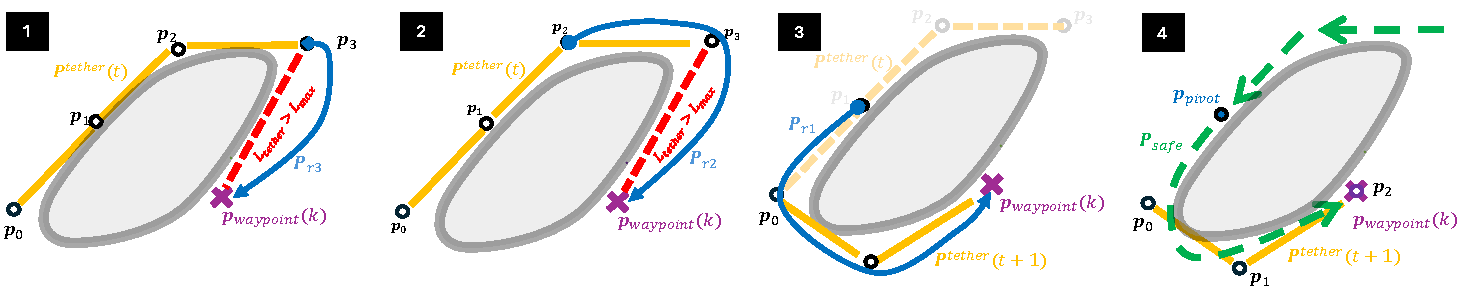
\includegraphics[width=\textwidth]{EA-Planner/figures/planner.pdf}
    \caption{De-entanglement path search process. 
    (1) Entanglement detection: following the path from node \( \mathbf{p}_3 \), denoted as \( \mathbf{P}_{r_3} \), causes the tether length \( L_{\text{tether}} \) to exceed the maximum allowed length \( L_{\text{max}} \); 
    (2) a backward recovery search is initiated from node \( \mathbf{p}_2 \) along the tether trajectory \( \mathbf{P}_{tether}(t) \), but the resulting path yields no improvement in tether length; 
    (3) continuing the search further back to node \( \mathbf{p}_1 \) leads to a feasible path and an updated, valid tether configuration; 
    (4) the final planned safe path \( \mathbf{P}_{safe} \) (green) satisfies the tether constraint (\( L_{\text{tether}} \leq L_{\text{max}} \)), ensuring an entanglement-free configuration.}
    \label{fig:planner_search}
\end{figure*}
%%%%%%%%%%%%%%%%
%%%%%%%%%%%%%%%%




\subsection{Recovery Path Refinement and Execution}
The initially selected recovery path \( \mathbf{P}_{\text{recovery}} \) undergoes further refinement to enhance safety and smoothness before execution. This involves several steps:
\begin{enumerate}
    \item Centroid Offsetting: Points along \( \mathbf{P}_{\text{recovery}} \) are pushed slightly outwards, away from the path's geometric centroid, to increase clearance from potential obstacles near the path's center.
    \item Random Sampling Perturbation: Points are locally perturbed by sampling in random directions, seeking nearby collision-free states to potentially escape minor constraint violations or local minima.
    \item Polynomial Smoothing: A polynomial function (e.g., 3rd order) is fitted to segments of the path to generate a smoother trajectory, reducing sharp turns and improving dynamic feasibility.
\end{enumerate}
The resulting refined path is denoted as \( \mathbf{P}_{\text{safe}} \). The planner then checks if \( \mathbf{P}_{\text{safe}} \) is collision-free using the state validity checker. If the entanglement strategy is active and \( \mathbf{P}_{\text{safe}} \) is valid, the controller is directed to follow points sequentially along \( \mathbf{P}_{\text{safe}} \). Once the \ac{ROV} reaches the end of \( \mathbf{P}_{\text{safe}} \), the entanglement avoidance strategy is deactivated, and the planner reverts to nominal operation, targeting the next waypoint from the original list \( \mathbf{W} \). If \( \mathbf{P}_{\text{safe}} \) is found to be invalid (e.g., due to collisions introduced during refinement), the system continues targeting the original waypoint \( \mathbf{p}_{\text{waypoint}}(k) \), relying on lower-level collision avoidance or requiring further planning cycles. 

The core logic can be summarized in the following algorithms. Algorithm~\ref{alg:main_loop} outlines the main planning cycle, Algorithm~\ref{alg:search_alternative} details the search for the recovery path, and Algorithm~\ref{alg:refine_path} describes the path refinement process.














%%%%%%%%%%%%%%%%%%%%%%%%%%%%%%%%%%%%%%%%%%
%%%%%%%%%%%%%%%%%%%%%%%%%%%%%%%%%%%%%%%%%%
%%%%%%%%%%%%%%%%%%%%%%%%%%%%%%%%%%%%%%%%%%













